\documentclass[main.tex]{subfiles}
\begin{document}
	
	In this section, we present the initial results of our implementation of the GRIN framework. The measurements presented here can only be considered preliminary, given the compiler needs further work to be comparable to systems like the Glasgow Haskell Compiler or the Idris compiler~\cite{idris}. Nevertheless, these statistics are still relevant, since they provide valuable information about the effectiveness of the optimizer.
	
	\subsection{Measured programs}
	
	%TODO: include code of Length
	The measurements were taken using the Idris front end and LLVM back end of the compiler. Each test program --- besides ``Length" --- was adopted from the book \textit{Type-driven development with Idris}~\cite{tdd-idris} by Edwin Brady. These are small Idris programs demonstrating a certain aspect of the language.
	
	``Length" is an Idris program, measuring the length of a list containing the natural numbers from 1 to 100. This example was mainly constructed to test how the dead data elimination pass can transform the inner structure of a list into a simple natural number (see Section~\ref{sec:dde}).
	
	\subsection{Measured metrics}
	
	Each test program went trough the compilation pipeline described in Section~\ref{sec:idris-front-end}, and measurements were taken at certain points during the compilation. The programs were subject to three different types of measurements.
	
	\vspace{0.25cm}
	\begin{itemize}
		\item Static, compile time measurements of the GRIN code.
		\item Dynamic, runtime measurements of the interpreted GRIN code.
		\item Dynamic, runtime measurements of the executed binaries.
	\end{itemize}
	\vspace{0.25cm}

	The compile time measurements were taken during the GRIN optimization passes, after each transformation. The measured metrics were the number of \pilcode{store}s, \pilcode{fetch}es and function definitions. These measurements ought to illustrate how the GRIN code becomes more and more efficient during the optimization process. The corresponding diagrams for the static measurements are Diagrams~\ref{diagram:length-stats-ct}~to~\ref{diagram:reverse-stats-ct}. On the horizontal axis, we can see the indices of the transformations in the pipeline, and on the vertical axis, we can see the number of the corresponding syntax tree nodes. Reading these diagram from left to right, we can observe the continuous evolution of the GRIN program throughout the optimization process.
	
	The runtime measurements of the interpreted GRIN programs were taken three points during the compilation process. First, right after the GRIN code is generated from the Idris byte code; second, after the regular optimization passes; and finally, at the end of the entire optimization pipeline. As can be seen on Figure~\ref{fig:measurement-pipeline}, the regular optimizations are run a second time right after the dead data elimination pass. This is because the DDE pass can enable further optimizations. To clarify, the third runtime measurement of the interpreted GRIN program was taken after the second set of regular optimizations. The measured metrics were the number of executed function calls, case pattern matches, \pilcode{store}s and \pilcode{fetch}es. The goal of these measurements is to compare the GRIN programs at the beginning and at the end of the optimization pipeline, as well as to evaluate the efficiency of the dead data elimination pass. The corresponding diagrams for these measurement are Diagrams~\ref{diagram:length-stats-rt}~to~\ref{diagram:reverse-stats-rt}.

	The runtime measurements of the binaries were taken at the exact same points as the runtime measurements of the interpreted GRIN code. Their goal is similar as well, however they ought to compare the generated binaries instead of the GRIN programs. The measured metrics were the size of the binary, the number of executed user-space instructions, stores and loads. The binaries were generated by the LLVM back end described in Section~\ref{subsec:llvm-back-end} with varying flags for the LLVM Optimizer.
	
	\subsection{Measurement setup}
	
	% DONE
	%- idris FR, LLVM BE
	%- small programs from TDD
	%- simple code generation
	%- no GC
	%- pipeline setup
	
	% TODO
	%- cant compare to IC
	%- compile & runtime stats for GRIN IR
	%- runtime stats for binary
	%- optimization levels?
	
	
	\begin{figure}
		\hspace{-0.5cm}
		\renewcommand{\figurename}{Diagram}
		\caption{Length - GRIN statistics}
		\label{diagram:length-stats}
		\addtocounter{figure}{-1}
		\begin{minipage}{0.5\textwidth}
			\subcaption{Runtime}
			\label{diagram:length-stats-rt}
			\resizebox{\width}{7cm}{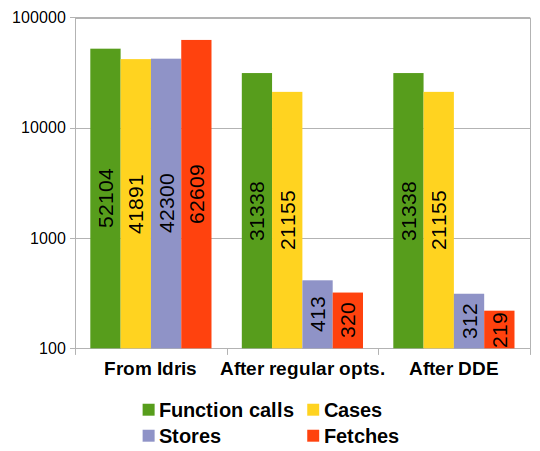
\includegraphics[scale=0.55]{length-runtime.png}}
		\end{minipage}
		\begin{minipage}{0.5\textwidth}
			\subcaption{Compile time}
			\label{diagram:length-stats-ct}
			\resizebox{\width}{7cm}{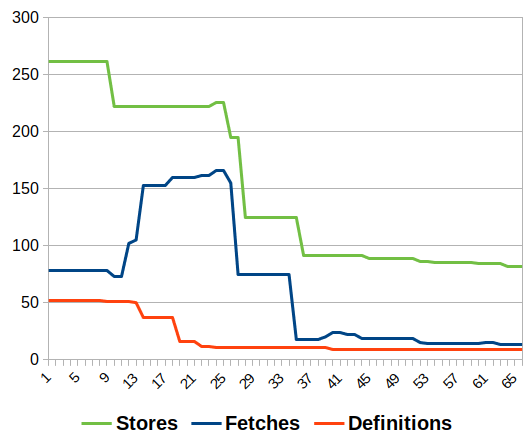
\includegraphics[scale=0.55]{length-compile-time.png}}
		\end{minipage}
	\end{figure}

	\begin{figure}
		\hspace{-0.5cm}
		\renewcommand{\figurename}{Diagram}
		\caption{Exact length - GRIN statistics}
		\label{diagram:exact-length-stats}
		\addtocounter{figure}{-1}
		\begin{minipage}{0.5\textwidth}
			\subcaption{Runtime}
			\label{diagram:exact-length-stats-rt}
			\resizebox{\width}{7cm}{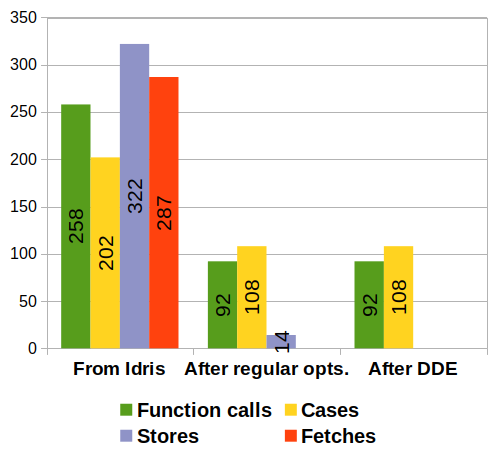
\includegraphics[scale=0.55]{exact-length-runtime.png}}
		\end{minipage}
		\begin{minipage}{0.5\textwidth}
			\subcaption{Compile time}
			\label{diagram:exact-length-stats-ct}
			\resizebox{\width}{7cm}{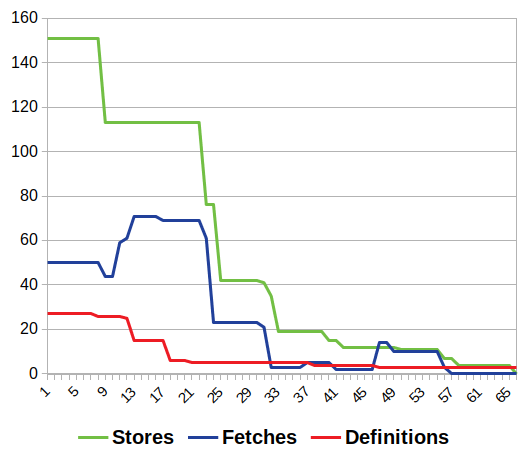
\includegraphics[scale=0.55]{exact-length-compile-time.png}}
		\end{minipage}
	\end{figure}
	
	\begin{figure}
		\hspace{-0.5cm}
		\renewcommand{\figurename}{Diagram}
		\caption{Type level functions - GRIN statistics}
		\label{diagram:tyfuns-stats}
		\addtocounter{figure}{-1}
		\begin{minipage}{0.5\textwidth}
			\subcaption{Runtime}
			\label{diagram:tyfuns-stats-rt}
			\resizebox{\width}{7cm}{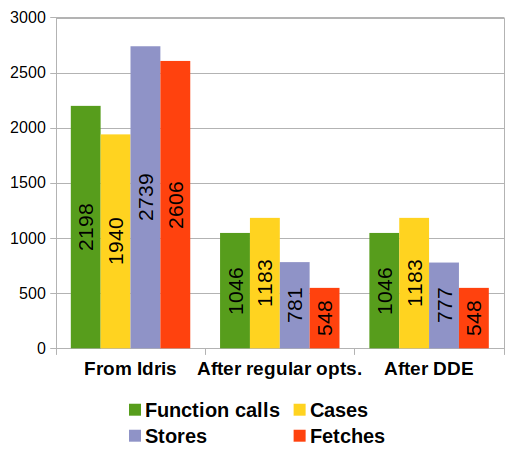
\includegraphics[scale=0.55]{tyfuns-runtime.png}}
		\end{minipage}
		\begin{minipage}{0.5\textwidth}
			\subcaption{Compile time}
			\label{diagram:tyfuns-stats-ct}
			\resizebox{\width}{7cm}{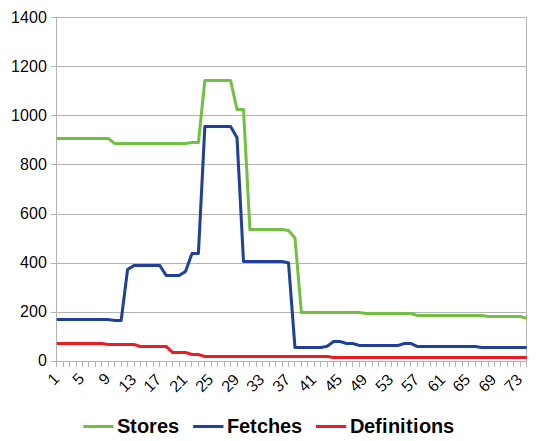
\includegraphics[scale=0.55]{tyfuns-compile-time.png}}
		\end{minipage}
	\end{figure}
	
	\begin{figure}
		\hspace{-0.5cm}
		\renewcommand{\figurename}{Diagram}
		\caption{Reverse - GRIN statistics}
		\label{diagram:reverse-stats}
		\addtocounter{figure}{-1}
		\begin{minipage}{0.5\textwidth}
			\subcaption{Runtime}
			\label{diagram:reverse-stats-rt}
			\resizebox{\width}{7cm}{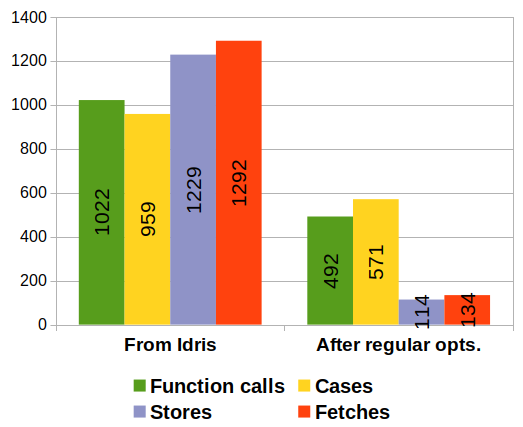
\includegraphics[scale=0.55]{reverse-runtime.png}}
		\end{minipage}
		\begin{minipage}{0.5\textwidth}
			\subcaption{Compile time}
			\label{diagram:reverse-stats-ct}
			\resizebox{\width}{7cm}{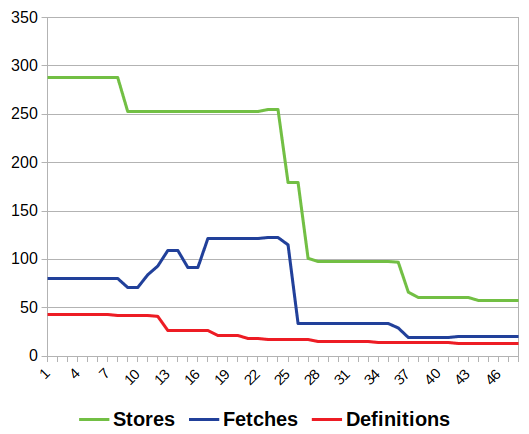
\includegraphics[scale=0.55]{reverse-compile-time.png}}
		\end{minipage}
	\end{figure}
	
	\begin{center}
		\begin{minipage}{0.6\linewidth}
			\captionof{table}{Length - binary statistics}
			\label{table:length-binary-results}
			\begin{tcolorbox}[tab2,tabularx={l||r|r|r|r}]
				Stage                 & Size  & Instructions & Stores & Loads      \\
				\hline\hline
				\pilcode{normal-O0}   & 23928 & 769588 & 212567 & 233305 \\\hline
				\pilcode{normal-O3}   & 23928 & 550065 & 160252 & 170202 \\\hline
				\pilcode{regular-opt} & 19832 & 257397 & 14848  & 45499  \\\hline
				\pilcode{dde-O0}      & 15736 & 256062 & 14243  & 45083  \\\hline
				\pilcode{dde-O3}      & 15736 & 284970 & 33929  & 54555  \\
			\end{tcolorbox}	
		\end{minipage}
	\end{center}
	
	\begin{center}
		\begin{minipage}{0.58\linewidth}
			\captionof{table}{Exact length - binary statistics}
			\label{table:exact-length-binary-results}
			\begin{tcolorbox}[tab2,tabularx={l||r|r|r|r}]
				Stage                 & Size  & Instructions & Stores & Loads      \\
				\hline\hline
				\pilcode{normal-O0}   & 18800 & 188469 & 14852 & 46566 \\\hline
				\pilcode{normal-O3}   & 14704 & 187380 & 14621 & 46233 \\\hline
				\pilcode{regular-opt} & 10608 & 183560 & 13462 & 45214 \\\hline
				\pilcode{dde-O0}      & 10608 & 183413 & 13431 & 45189 \\\hline
				\pilcode{dde-O3}      & 10608 & 183322 & 13430 & 44226 \\
			\end{tcolorbox}	
		\end{minipage}
	\end{center}
	
	\begin{center}
		\begin{minipage}{0.58\linewidth}
			\captionof{table}{Type level functions - binary statistics}
			\label{table:tyfuns-binary-results}
			\begin{tcolorbox}[tab2,tabularx={l||r|r|r|r}]
				Stage                 & Size  & Instructions & Stores & Loads      \\
				\hline\hline
				\pilcode{normal-O0}   & 65128 & 383012 & 49191 & 86754 \\\hline
				\pilcode{normal-O3}   & 69224 & 377165 & 47556 & 84156 \\\hline
				\pilcode{regular-opt} & 36456 & 312122 & 34340 & 71162 \\\hline
				\pilcode{dde-O0}      & 32360 & 312075 & 34331 & 70530 \\\hline
				\pilcode{dde-O3}      & 28264 & 309822 & 33943 & 70386 \\
			\end{tcolorbox}	
		\end{minipage}
	\end{center}
	
	\begin{center}
		\begin{minipage}{0.62\linewidth}
			\captionof{table}{Reverse - binary statistics}
			\label{table:reverse-binary-results}
			\begin{tcolorbox}[tab2,tabularx={l||r|r|r|r}]
				Stage                 & Size  & Instructions & Stores & Loads      \\
				\hline\hline
				\pilcode{normal-O0}      & 27112 & 240983 & 25018 & 58253 \\\hline
				\pilcode{normal-O3}      & 31208 & 236570 & 23808 & 56617 \\\hline
				\pilcode{regular-opt-O0} & 14824 & 222085 & 19757 & 53125 \\\hline
				\pilcode{regular-opt-O3} & 14824 & 220837 & 19599 & 52827 \\
			\end{tcolorbox}	
		\end{minipage}
	\end{center}

\end{document}